\section{Описание подхода}

TalkNet splits the text-to-spectrogram generation into two separate modules. The first module, the duration predictor, aligns input graphemes in time with respect to the audio features. The second module, the mel-spectrogram generator, produces mel-spectrograms from time-aligned input characters. We use feed-forward CNNs for both modules, so both training and inference are non-autoregressive. This allows for much faster training and inference compared to auto-regressive models. To train the grapheme duration predictor we extracted ground truth alignment from the CTC output of a pre-trained ASR model.  

\subsection{Ground truth grapheme duration extraction}

\begin{figure}[!ht]
\centering
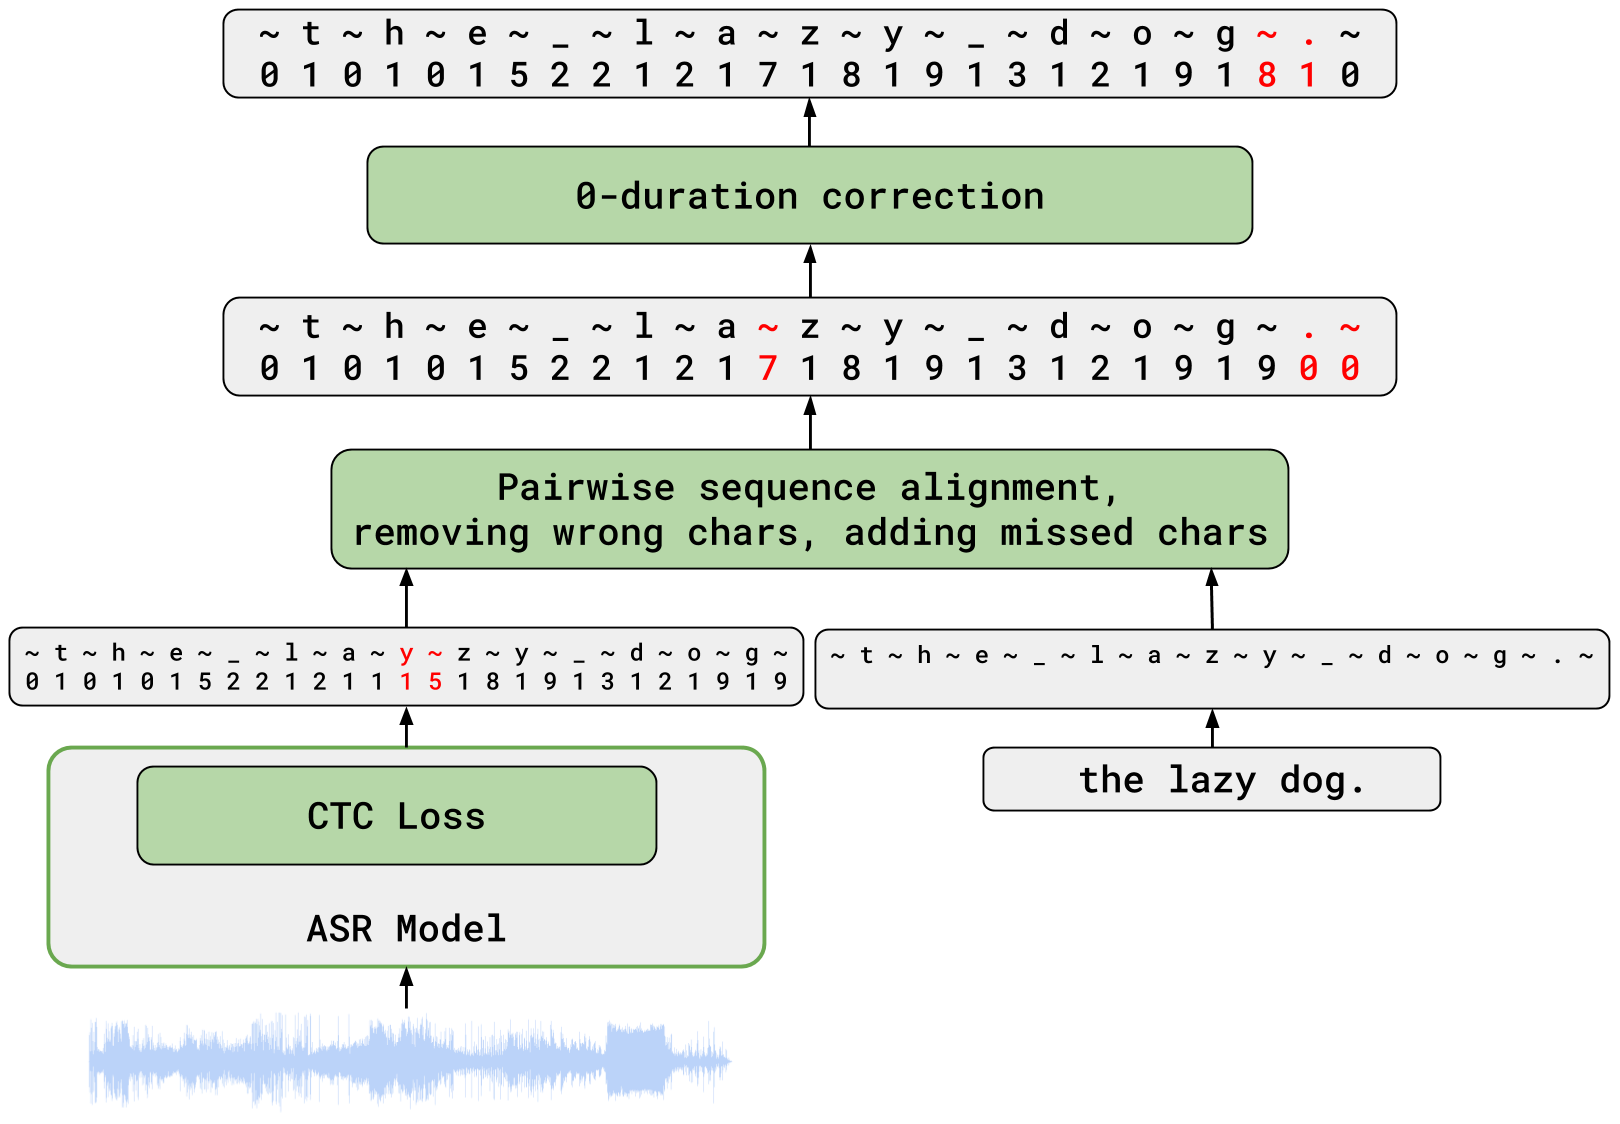
\includegraphics[width=1.0\textwidth]{images/alignment.png}
\caption{Grapheme duration extraction from CTC output. We use $\sim$ to denote the blank symbol.}
\label{fig:alignment}
\end{figure}

The central idea behind TalkNet is to use a CTC-based ASR model to extract grapheme alignments. CTC assigns a probability to each of characters from the alphabet, with an auxiliary blank symbol $\sim$. The blank symbol acts as an intermediate state between two neighboring graphemes, and its duration corresponds to the length of the transition from one character to another. For each time step, we choose the most likely character from the CTC output. Because the CTC output is imperfect, we align it with the ground truth text using the \textit{pairwise2} function from the Biopython~\cite{biopython} package. We then remove all the incorrect characters in the CTC output, adding their duration to the nearest blank, and add the missing characters and set their duration to $0$. Next, for all the characters with predicted duration 0,  we set the duration to 1 by subtracting 1 from the near biggest blank to keep the sum of all grapheme durations equal to the length of a mel-spectrogram (see Figure~\ref{fig:alignment}).

To obtain the ground truth grapheme duration we use QuartzNet15x5~\cite{quartznet} with a minor modification: we set the stride in the first convolutional layer to $1$ to make the length of the CTC output equal to the length of the mel-spectrogram. Apart from this, we keep all punctuation intact while tokenizing the text to let CTC handle punctuation alignment as well. We train QuartzNet on LibriTTS~\cite{libritts}. We achieve a CER of $4.51\%$ on LibriTTS test-clean and $3.54\%$ on the LJSpeech test set. The alignment obtained from CTC is used to train the grapheme duration predictor.

\subsection{Grapheme duration predictor}

This model predicts the length of the mel-spectrogram part corresponding to each gra\-pheme in the input including punctuation. First, the grapheme duration predictor inserts a blank symbol $\sim$ between every two input characters. Next, it predicts the duration for each input character. We expand the sequence of input characters by repeating each character according to the predicted duration  (Figure~\ref{fig:durs}).

\begin{figure}[!ht]
\centering
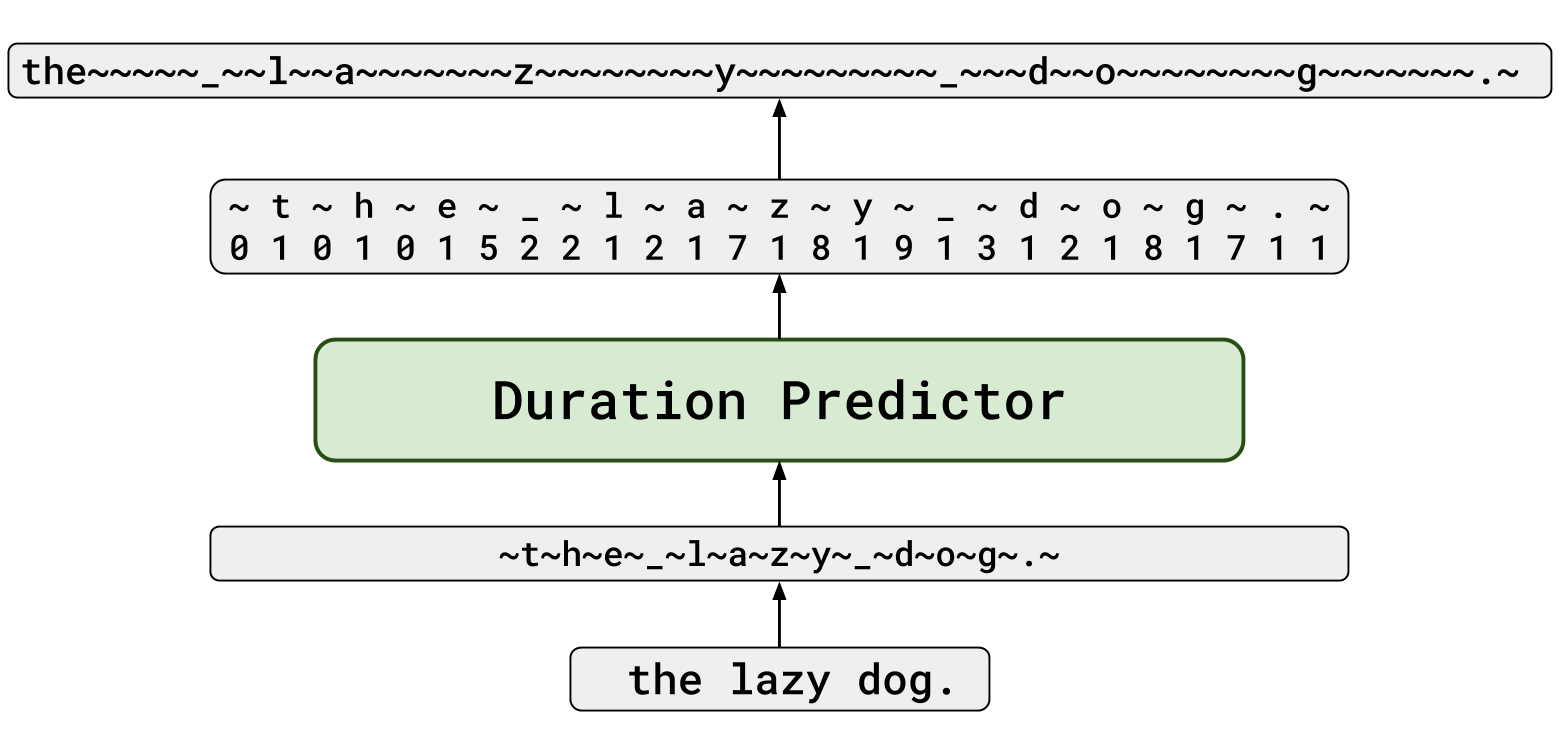
\includegraphics[width=1.0\linewidth]{images/durs.png}
\caption{Grapheme duration prediction.}
\label{fig:durs}
\end{figure}

The grapheme duration predictor model is a 1D time channel separable convolutional NN based on QuartzNet architecture~\cite{quartznet}. The model has $5$ residual blocks with 5 sub-blocks per block. A sub-block consists of a 1D time-channel separable convolution, a 1x1 pointwise convolutions, batch norm, ReLU, and dropout (see Figure~\ref{fig:qn-block}). There are two additional layers: the grapheme embedding layer, and a $1x1$ convolutional layer before loss function (see Table~\ref{tab:durs-model}).

\begin{figure}[!ht]
\centering
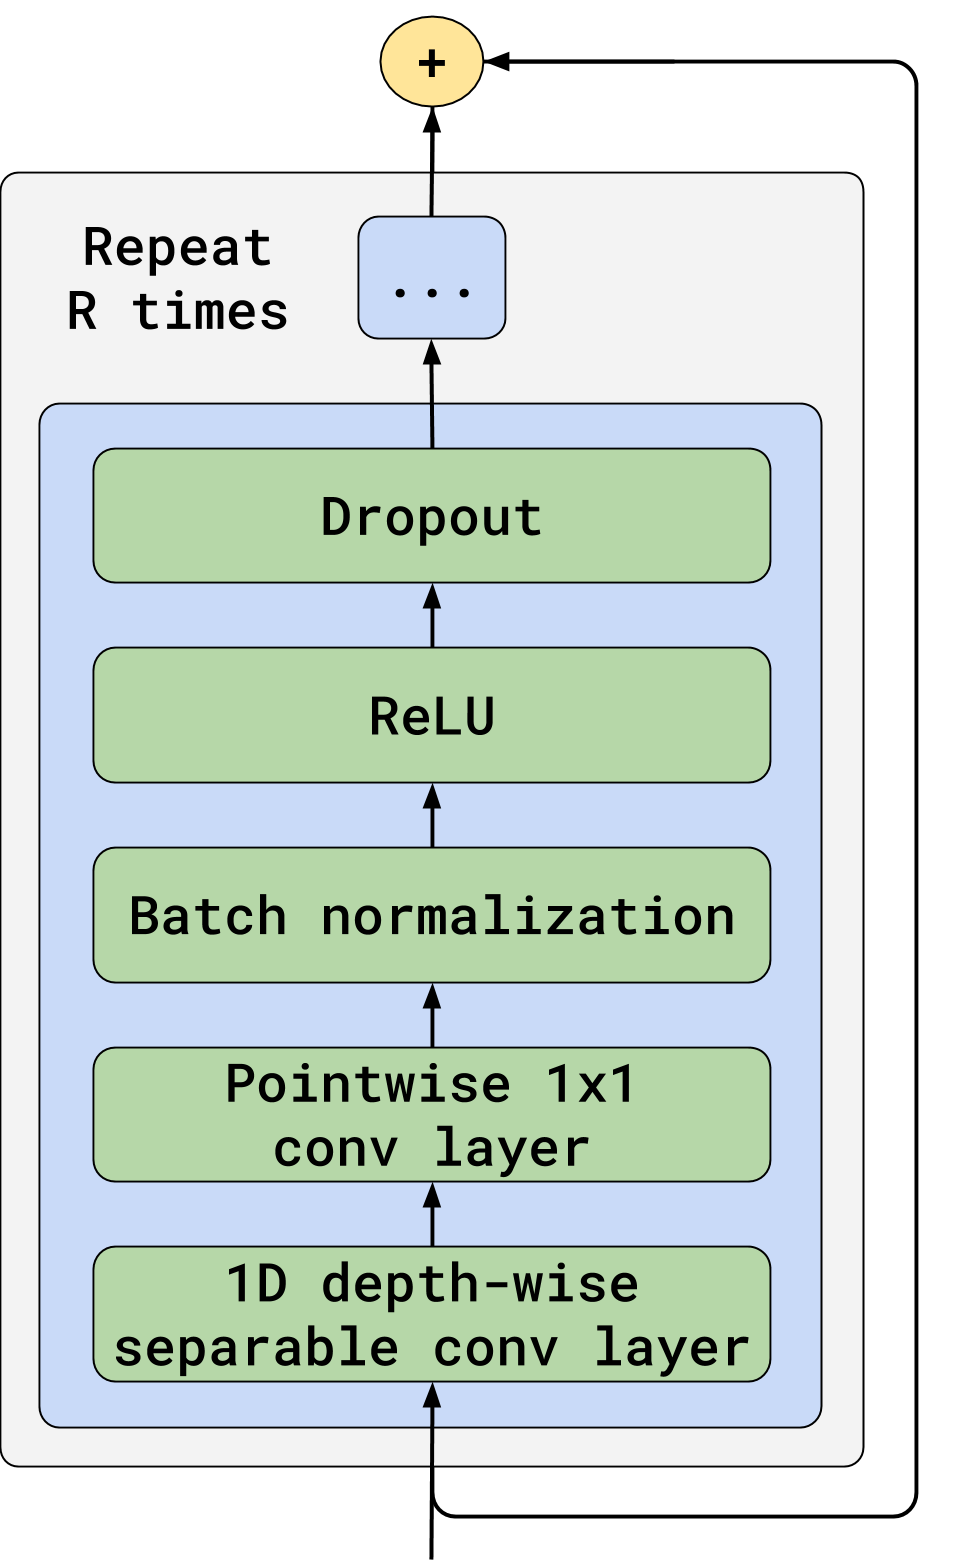
\includegraphics[width=0.8\linewidth]{images/qn-block.png}
\caption{Basic QuartzNet block. Both grapheme duration predictor and mel-spectrogram generator are 1D time-channel convolutional networks based on QuartzNet~\cite{quartznet}.}
\label{fig:qn-block}
\end{figure}

We train a duration predictor using $L_2$ loss with logarithmic targets, similar to~\cite{fastspeech}. We also tried cross-entropy (XE) loss with each class corresponding to the character duration. We used a log scale for large durations since grapheme duration distribution has a long tail (Figure~\ref{fig:durs-dist}). Cross entropy has slightly higher accuracy (see Table~\ref{tab:durs-results}). We choose $L2$ since a speech generated with L2 loss got slightly higher mean-opinion-score (MOS) in our evaluation studies.

\begin{figure}[!ht]
\centering
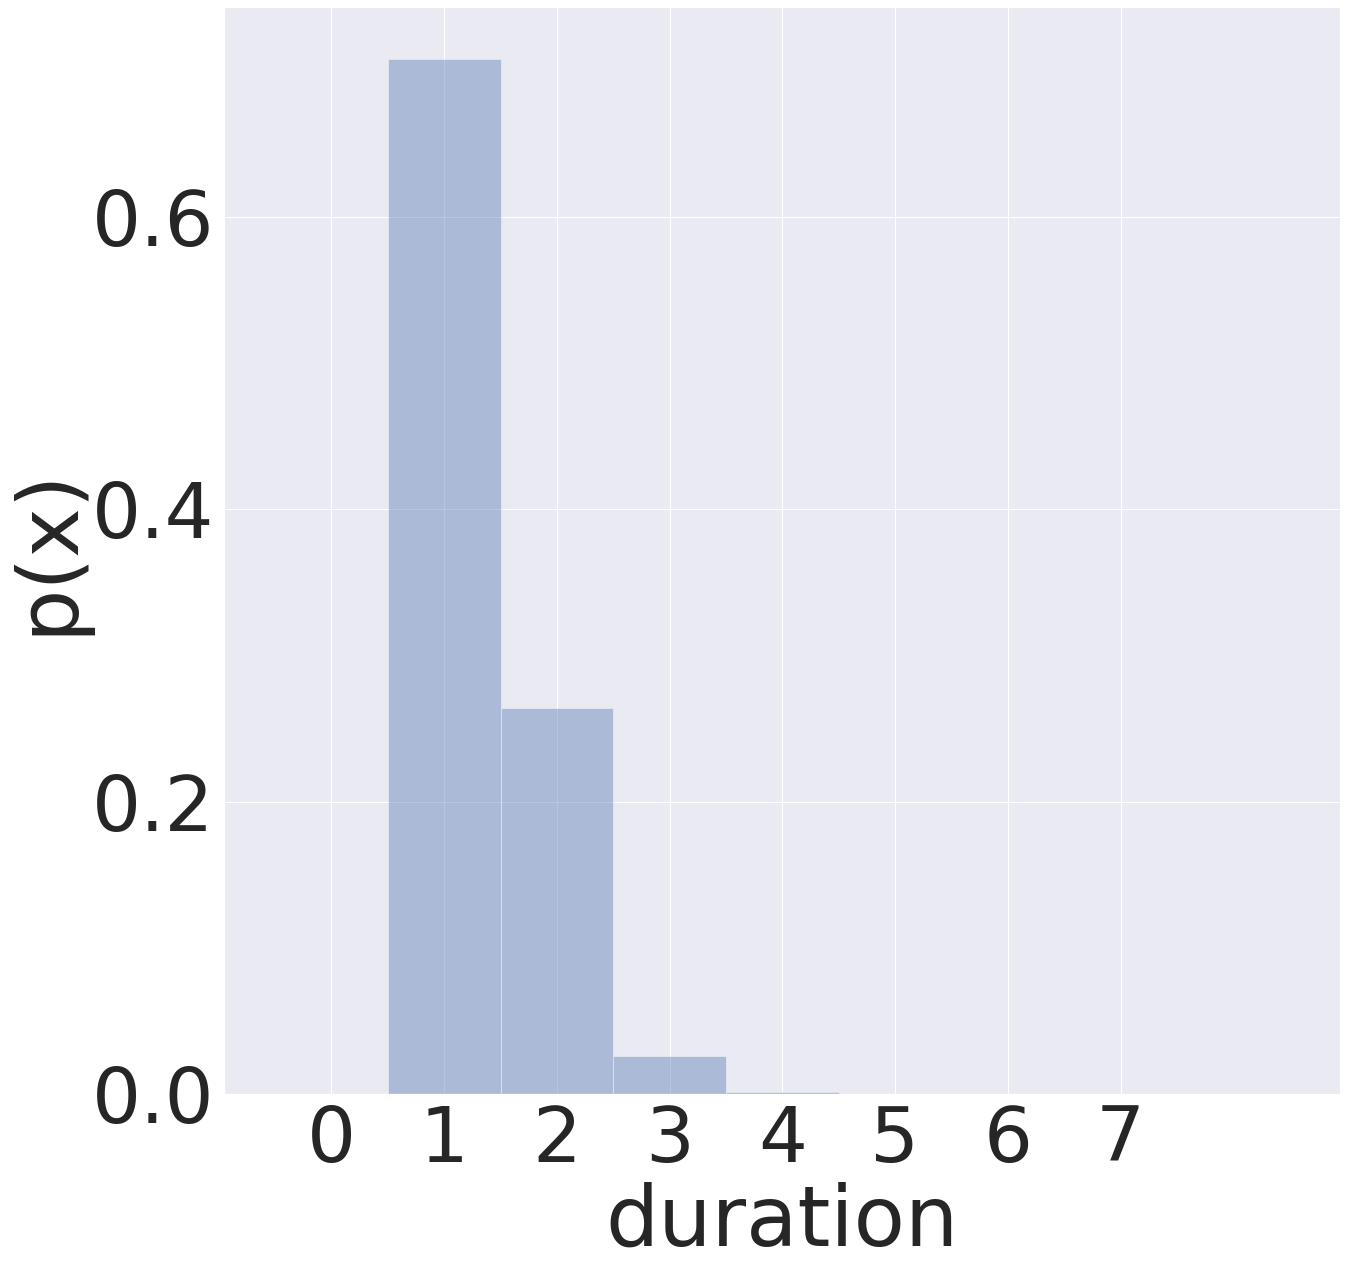
\includegraphics[width=.48\linewidth]{images/durs-dist.png}
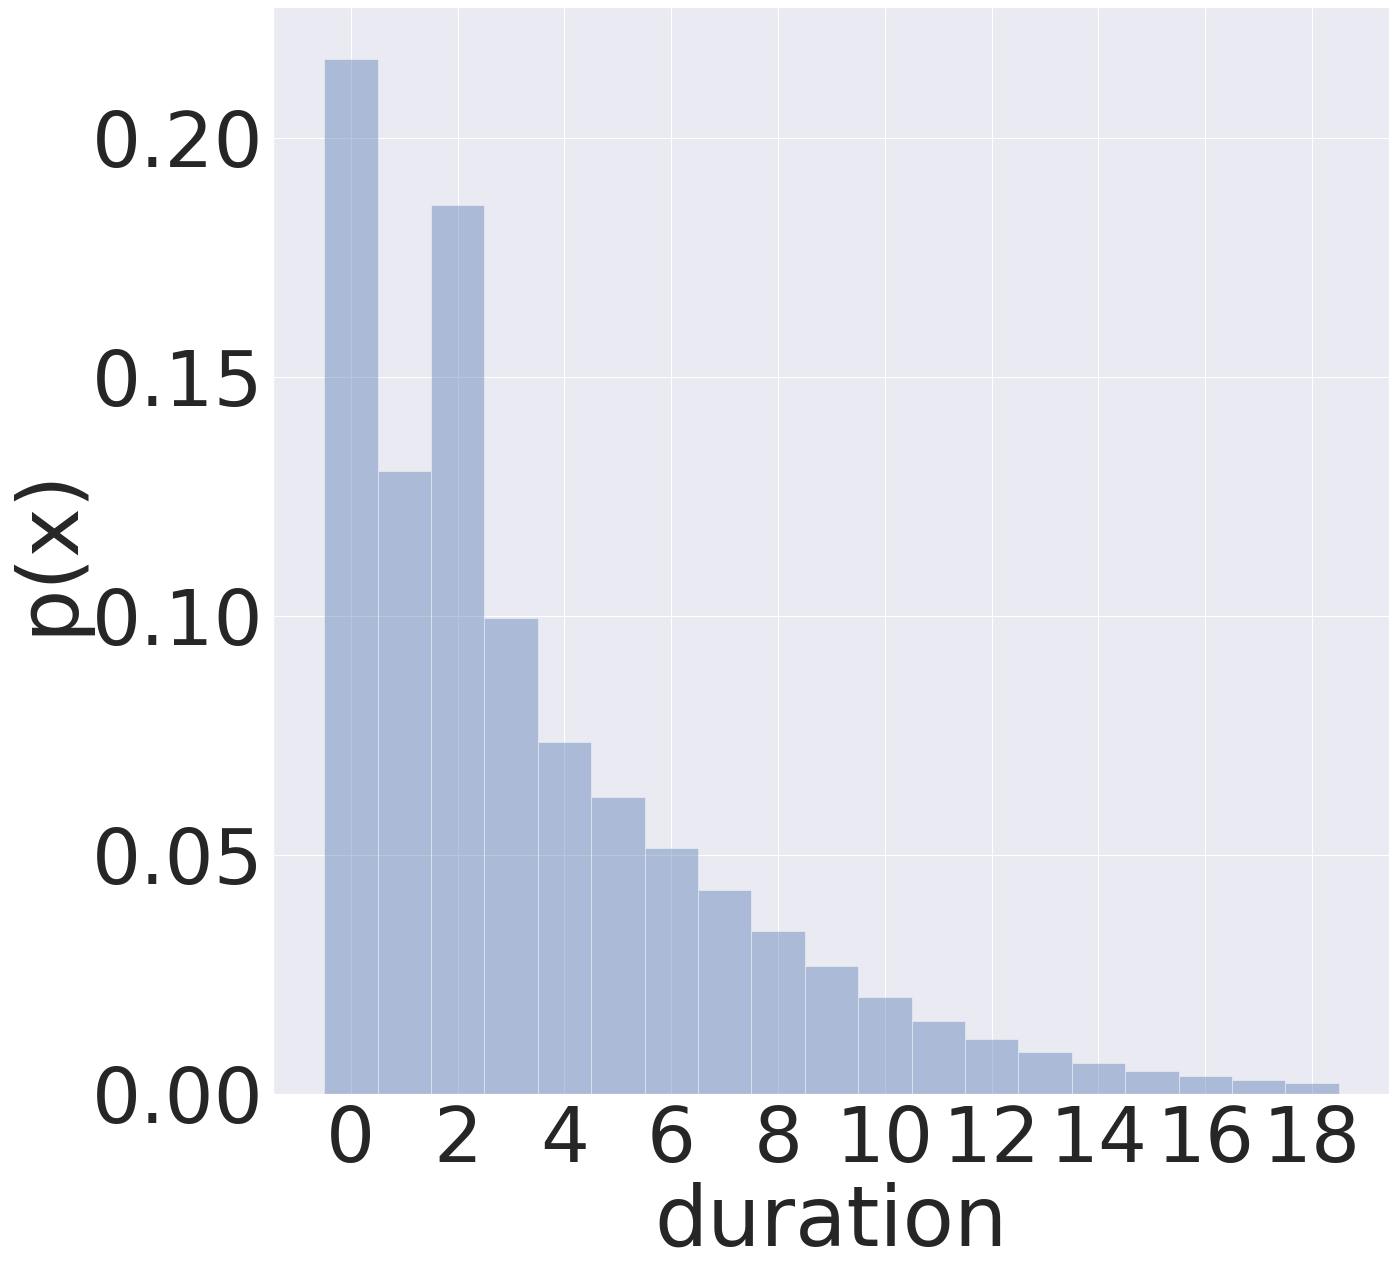
\includegraphics[width=.48\linewidth]{images/blanks-dist.png}
\caption{The duration's distribution for characters (left) and for blanks (right) based on CTC output for LJSpeech dataset. The maximum duration for characters is $7$, and for blanks -- $493$.}
\label{fig:durs-dist}
\end{figure}

\begin{table}[!ht]
\centering
\scalebox{1.0}{
\begin{tabular}{c c c c c} 
\toprule
\textbf{Block} &
\textbf{\thead{\# Sub\\Blocks}} &
\textbf{\thead{\# Output\\Channels}} &
\textbf{Kernel Size} &
\textbf{Dropout} \\
\midrule
Embed & 1 & 64  & 1 & 0.0  \\
Conv1 & 3 & 256 & 3 & 0.1  \\
$B_1$ & 5 & 256 & 5 & 0.1  \\
$B_2$ & 5 & 256 & 7 & 0.1  \\
$B_3$ & 5 & 256 & 9 & 0.1  \\
$B_4$ & 5 & 256 & 11 & 0.1 \\
$B_5$ & 5 & 256 & 13 & 0.1 \\
Conv2 & 1 & 512 & 1 & 0.1  \\
Conv3 & 1 & $32$ & 1 & 0.0 \\
\midrule
\textbf{Params, M} & & & & \textbf{2.3} \\
\bottomrule
\end{tabular}
}
\caption{Grapheme duration predictor is based on QuartzNet 5x5.}
\label{tab:durs-model}
\end{table}

\begin{table}[!ht]
\centering
\scalebox{1.0}{
\begin{tabular}{c c c c c c c} 
\toprule
\textbf{Method} &
\textbf{MSE} &
\textbf{Accuracy, $\%$} &
$\mathbf{|P - T| \leq 1}$ &
$\mathbf{|P - T| \leq 3}$\\
\midrule
$L_2$ & 7.81 & 67.69 & 91.90 & 97.17 \\
XE & 10.46 & 69.42 & 92.90 & 97.40 \\
\bottomrule
\end{tabular}
}
\caption{Duration's predictor results, LJSpeech test set. $P$ -- predicted, $T$ -- target.}
\label{tab:durs-results}
\end{table}

\subsection{Mel-spectrogram generator}

The second module generates mel-spectrogram from the expanded text. The mel-spectro\-gram generator is a 1D convolutional network based on the same QuartzNet architecture. It has $9$ blocks with 5 sub-blocks (see Table~\ref{tab:mels-model}). The mel-spectrogram generator was trained with a mean square error (MSE) loss.

Instead of allocating a separate embedding for blank symbol, we use a linear combination of embeddings for the neighboring graphemes. Namely, if the blank symbol $\sim$ is located between the  characters $a$ and $b$ and the blank duration is $d$, then the embedding $E$ for the blank symbol located at the distance $t$ from $a$ would be $E(\sim, t) = \dfrac{d+1-t}{d+1} \cdot E(a) + \dfrac{t}{d+1} \cdot E(b)$.

\begin{table}[!ht]
\centering
\scalebox{0.85}{
\begin{tabular}{c c c c c} 
 \toprule
  \textbf{Block} &
  \textbf{\thead{\# Sub\\Blocks}} &
  \textbf{\thead{\# Output\\Channels}} &
  \textbf{Kernel Size} &
  \textbf{Dropout} \\
 \midrule
Embed & 1 & 256 & 1 & 0.0 \\
Conv1 & 3 & 256 & 3 & 0.0 \\
$B_1$ & 5 & 256 & 5 & 0.0 \\
$B_2$ & 5 & 256 & 7 & 0.0 \\
$B_3$ & 5 & 256 & 9 & 0.0 \\
$B_4$ & 5 & 256 & 13 & 0.0 \\
$B_5$ & 5 & 256 & 15 & 0.0 \\
$B_6$ & 5 & 256 & 17 & 0.0 \\
$B_7$ & 5 & 512 & 21 & 0.0 \\
$B_8$ & 5 & 512 & 23 & 0.0 \\
$B_9$ & 5 & 512 & 25 & 0.0 \\
Conv2 & 1 & 1024 & 1 & 0.0 \\
Conv3 & 1 & 80 & 1 & 0.0 \\
\midrule
\textbf{Params, M} & & & & \textbf{8.5} \\
\bottomrule
\end{tabular}
}
\caption{Mel-spectrogram generator is based on QuartzNet~9x5.}
\label{tab:mels-model}
\end{table}